\section{Localisation}
The localisation for 2009 was based on the Unscented Kalman Filter (UKF) used in 2008 !REFERENCE!. A number of extensions were 
made to improve upon the previous years implementation. These changes were made to both include new information that was available due to advances in vision, as well as to make use of ambiguous data that was not previously usable.\\

\subsection{Multiple Models}
The current robocup field contains many ambiguous points of reference as can be seen in \autoref{fig:LocalisationPoints}. When multiple ambiguous points are found it is possible to use a simple decision tree to determine which objects these are, however there are often times where this is not possible. The UKF was therefore extended to incorperate multiple models to allow for the use of ambiguous measurements.\\

The basic idea is that when an ambiguous object is seen e.g. a yellow goal post, we can determine that there are a number of possible fixed objects that could have been seen, in this example the left yellow post or the right yellow post. Using a multiple models approach the current model cloned to create as many models as there are options, in our example two. One model is then updated with the first option the next model with the second and so forth.\\

As these updates are done an \emph{alpha} variable is modified depending on how well the update fits the previous model. The larger the discrepancy the more the alpha value is reduced. Therefore the model with the largest alpha value following the update can be deemed to have been updated with the most likely option and therefore will be the most correct model. This process can be repeated for multiple ambiguous options and therefore the results of all possible combinations can be found.
If this process were repeated again and again, we would end up with an exponentially growing collection of models. Therefore it is also necessary to merge these models, combining two models into one. Merging is done so that information is not lost. Models are merged based on the following metric !REFERENCE!.\\

\begin{figure}[!h]
\begin{center}
   \leavevmode
    \scalebox{0.5} {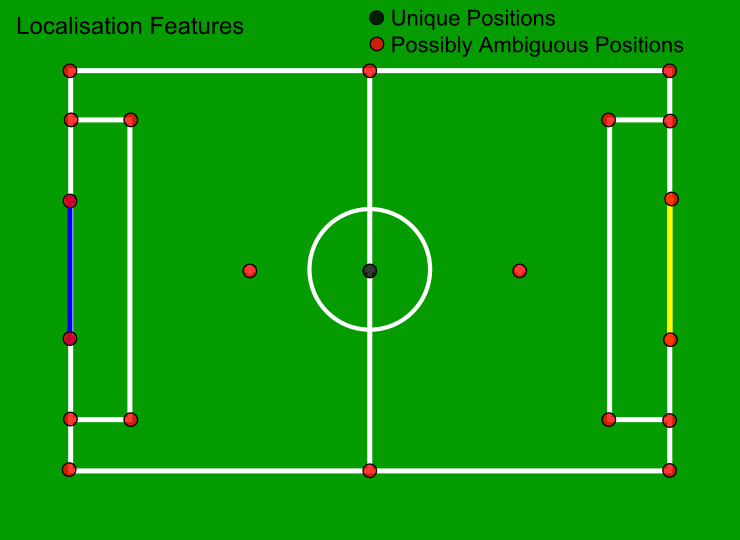
\includegraphics{figs/LocalisationPoints.png} }
    \caption{Available localisation landmarks}
    \label{fig:LocalisationPoints}
\end{center}
\end{figure}

